\documentclass{beamer}

\usepackage[utf8]{inputenc}
\usepackage{epigraph}
\usepackage{tikz}
\usepackage{csquotes}

\usetikzlibrary{patterns, arrows, cd, positioning, backgrounds, fit, decorations.pathmorphing, shapes.misc, calc, matrix, decorations.pathreplacing, external}
\tikzset{%
  node/.style={draw, minimum size=12mm, inner sep=0mm, circle, fill=gray!50},
  edge/.style={thick},
  move/.style={->},
  brace/.style={
    decorate,
    decoration={brace,amplitude=10pt,mirror},
  },
  table nodes/.style={
    rectangle,
    draw=black,
    align=center,
    minimum height=7mm,
    text depth=0.5ex,
    text height=2ex,
    inner xsep=0pt,
    outer sep=0pt,
    inner sep=0pt
  },
  table/.style={
    matrix of nodes,
    row sep=-0.5pt,
    column sep=-0.5pt,
    nodes={
      table nodes
    }
  }
}


\usetheme{metropolis}
\metroset{numbering=fraction}

\title{A Grimm idea}
\subtitle{Exploring graphs with pebbles}
\author{Christoph Welzel}
\institute{Logik und Theorie diskreter Systeme, RWTH Aachen}

\begin{document}
\maketitle
\begin{frame}
  \frametitle{Motivation}
  \begin{itemize}
    \item Traversing Brobdingnagian graphs
    \item[$\rightarrow$] Web crawlers
    \item Agent moves over vertices along edges
    \item[$\Rightarrow$] Memory efficient agents
  \end{itemize}
\end{frame}

\begin{frame}
  \frametitle{Agents}
  \begin{quotation}
    Und als der volle Mond aufgestiegen war, so nahm Hänsel sein
    Schwesterchen an der Hand und ging den Kieselsteinen nach, die schimmerten
    wie neu geschlagene Batzen und zeigten ihnen den Weg.
  \end{quotation}
  \vspace{-0.5cm}
  \flushright{Brüder Grimm}
  \vspace{-0.5cm}
  \flushright{\emph{Hänsel und Gretel}}
  \begin{itemize}
    \item Agent carries set of markers $\rightarrow$ pebbles
    \item Leave pebbles on vertices
  \end{itemize}
\end{frame}

\begin{frame}
  \frametitle{Brobdignagian graphs}
  \begin{columns}
    \column{0.5\textwidth}
    \begin{itemize}
      \item Indistinguishable vertices
      \item Bounded degree ($\Delta$)
      \item Edges can locally enumerated $\left\{0,\dots,\Delta-1\right\}$
        (Port)
      \item Agent is aware of:
        \begin{enumerate}
          \item Degree  of vertex
          \item Pebbles placed on vertex
          \item Pebbles carried by agent
          \item Port    agent entered vertex
        \end{enumerate}
    \end{itemize}
    \column{0.5\textwidth}
    \begin{center}
      \resizebox{\textwidth}{!}{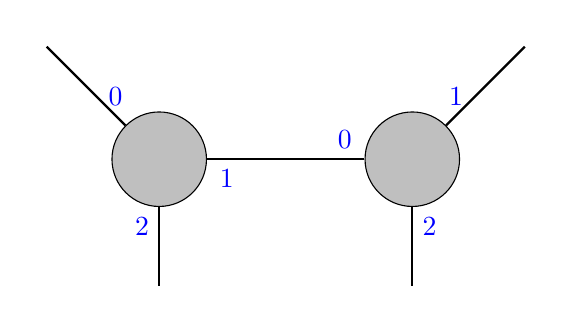
\begin{tikzpicture}
  \node[node] (m1) {};
  \node[node,right=2cm of m1] (m2) {};

  \node[above left=of m1] (e1) {};
  \node[below=of m1] (e2) {};

  \node[above right=of m2] (e3) {};
  \node[below=of m2] (e4) {};

  \draw[edge] (m1) to node[very near start, above] {\textcolor{blue}{0}} (e1);
  \draw[edge] (m1) to node[near start, left] {\textcolor{blue}{2}} (e2);

  \draw[edge] (m2) to node[very near start, above] {\textcolor{blue}{1}} (e3);
  \draw[edge] (m2) to node[near start, right] {\textcolor{blue}{2}} (e4);
  
  \draw[edge] (m1) to node[very near start, below] {\textcolor{blue}{1}} node[very near end, above] {\textcolor{blue}{0}} (m2);
\end{tikzpicture}
}
    \end{center}
  \end{columns}
\end{frame}

\begin{frame}
  \frametitle{Exploration sequence}
  \begin{columns}
    \column{0.5\textwidth}
    \begin{itemize}
      \item Describe movement of agent by relative turns
      \item $e_{1},\dots, e_{n}$
      \item For a vertex $v$ with degree $d_{v}$ which is entered on port $p$
        is left through port $p + e_{i}\mod p$
      \item<2->[$\rightarrow$] Example:
        $\only<3-3>{\colorbox{green}}{1}\;,\only<4-4>{\colorbox{green}}{3}\;,
        \only<5-5>{\colorbox{green}}{2}\;,\only<6-6>{\colorbox{green}}{2}$
    \end{itemize}
    \column{0.5\textwidth}
    \begin{center}
      \resizebox{\textwidth}{!}{\begin{tikzpicture}
  \node[minimum size=12mm,inner sep=0mm, circle] (8) {};
  \node[node,right=of 8] (6) {};
  \node[node,right=of 6] (7) {};
  \node[node,below=of 8] (0) {};
  \node[node,below=of 6] (1) {};
  \node[node,below=of 7] (2) {};
  \node[node,below=of 0] (3) {};
  \node[node,below=of 1] (4) {};
  \node[node,below=of 2] (5) {};
  \node[node,above right=0.5cm and 1cm of 2] (8) {};
  \node[node,below right=0.5cm and 1cm of 2] (9) {};

  \draw[edge] (0) to node[very near start, above] {0} node[very near end, above] {1} (1);
  \draw[edge] (1) to node[very near start, below] {0} node[very near end, above] {1} (2);
  \draw[edge,bend right] (2.north west) to node[very near start, right] {0} node[very near end, above] {2} (0);
  \draw[edge] (0) to node[very near start, right] {1} node[very near end, left ] {0} (3);
  \draw[edge] (3) to node[very near start, above] {1} node[very near end, below] {1} (4);
  \draw[edge] (4) to node[very near start, below] {0} node[very near end, below] {1} (5);
  \draw[edge] (5) to node[very near start, above] {0} node[very near end, below] {2} (1);
  \draw[edge] (1) to node[very near start, left ] {3} node[very near end, left ] {2} (6);
  \draw[edge] (6) to node[very near start, above] {0} node[very near end, above] {1} (7);
  \draw[edge] (8) to node[very near start, above] {0} node[very near end, right] {0} (7);
  \draw[edge] (8) to node[very near start, above] {1} node[very near end, right] {2} (5);
  \draw[edge] (9) to node[very near start, below] {1} node[very near end, below] {3} (5);
  \draw[edge,bend right=20] (9) to node[very near start, below] {0} node[very near end, below] {1} (6);

  \begin{scope}[on background layer]%
      \node [fit=(0)] (layer) {};%
  \end{scope}
  \begin{scope}[on background layer]%
      \node [fit=(4)] (layer) {};%
  \end{scope}
  \only<3-3>{\begin{scope}[on background layer]%
      \node [fit=(0), fill=green!50] (layer) {};%
  \end{scope}}
  \only<4-4>{\begin{scope}[on background layer]%
      \node [fit=(3), fill=green!50] (layer) {};%
  \end{scope}}
  \only<5-5>{\begin{scope}[on background layer]%
      \node [fit=(4), fill=green!50] (layer) {};%
  \end{scope}}
  \only<6-6>{\begin{scope}[on background layer]%
      \node [fit=(3), fill=green!50] (layer) {};%
  \end{scope}}
  \only<7-7>{\begin{scope}[on background layer]%
      \node [fit=(4), fill=green!50] (layer) {};%
  \end{scope}}


\end{tikzpicture}
}
    \end{center}
  \end{columns}
\end{frame}

\begin{frame}
  \frametitle{Closed walk}
  \begin{theorem}
    A exploration sequence $(e_{1},\dots,e_{k})^{\ast}$ produces a closed walk.
  \end{theorem}
  \begin{itemize}
    \item Introduce triple $(v,l,i)$ with vertex $v$ is entered
      through port $l$ and $e_{i}$ is the next turn
    \item Note that there is exactly one $(v,l,i) \leadsto (v',l',i')$
    \item Furthermore assume $t_{1} = (v',l',i') \leadsto (v,l,i)$ and
      $t_{2} = (v'',l'',i'') \leadsto (v,l,i)$:
      \begin{itemize}
        \item $t_{1}$ and $t_{2}$ both entered $v$ through $l$: $v' = v''$
        \item $t_{1}$ and $t_{2}$ lead that $i$ is the next turn: $i' = i''$
        \item $l' + e_{i'} \mod d_{v'} = l'' + e_{i''} \mod d_{v''}$ and
          $l',l''\leq d_{v'} = d_{v''}$: $l' = l''$
      \end{itemize}
    \item Only finite triples, thus projection to vertices yields closed walk
  \end{itemize}
\end{frame}

\begin{frame}
  \frametitle{Exploring pebble machine}
  \alt<+>{
    \begin{theorem}[Reingold]
      There is an algorithm $A$ with $\mathcal{O}(n)$ space requirement
      producing a universal exploration sequence for every regular graph with
      $n$ vertices.
    \end{theorem}
  }{
    \begin{theorem}
      Thus, there is $(\mathcal{O}(1), 0, \mathcal{O}(\log n)$ that moves
      along a closed walk with $n$ distinct vertices (or explores the whole
      graph).
    \end{theorem}
  }
  \begin{columns}
    \column{0.5\textwidth}
    \begin{itemize}
      \item<3-> Establish 3-regularity
        \begin{itemize}
          \item Transform $v$ to $3\cdot d_{v}$ distinct vertices
          \item TODO: ADD BOUNDARY
        \end{itemize}
      \item<5-> Use $A$ and take first $k = 3n\cdot c$ ($c$ number of
        configurations $M_{A}$)
    \end{itemize}
    \column{0.5\textwidth}
    \uncover<4->{\resizebox{\textwidth}{!}{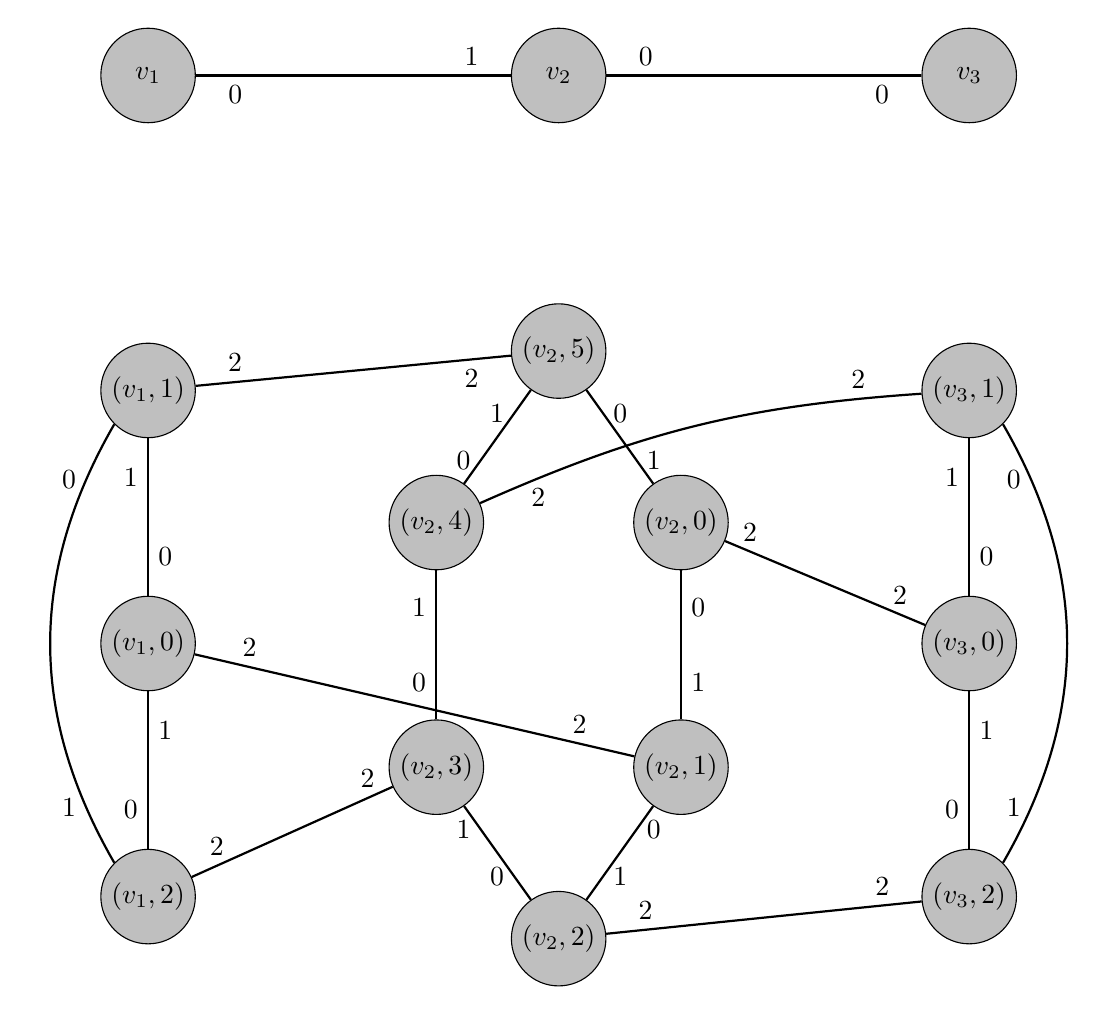
\begin{tikzpicture}
  \node[node] (m1) {$v_{1}$};
  \node[node] (m2) [right = 4cm of m1] {$v_{2}$};
  \node[node] (m3) [right = 4cm of m2] {$v_{3}$};

  \draw[edge] (m1) to node[below,very near start] {0} node[above,very near end] {1} (m2);
  \draw[edge] (m2) to node[above,very near start] {0} node[below,very near end] {0} (m3);

  \node[node] (r11) [below = 6cm of m1] {$(v_{1},0)$};
  \node[node] (r12) [above = 2cm of r11] {$(v_{1},1)$};
  \node[node] (r13) [below = 2cm of r11] {$(v_{1},2)$};

  \node[node] (l11) [below = 6cm of m3] {$(v_{3},0)$};
  \node[node] (l12) [above = 2cm of l11] {$(v_{3},1)$};
  \node[node] (l13) [below = 2cm of l11] {$(v_{3},2)$};

  \node       (anker) [below = 6.5cm of m2] {};
  \node[node] (mid0) [above right = 1cm and 1cm of anker] {$(v_{2},0)$};
  \node[node] (mid1) [below right = 1cm and 1cm of anker] {$(v_{2},1)$};
  \node[node] (mid2) [below = 3cm of anker] {$(v_{2},2)$};
  \node[node] (mid3) [below left = 1cm and 1cm of anker] {$(v_{2},3)$};
  \node[node] (mid4) [above left = 1cm and 1cm of anker] {$(v_{2},4)$};
  \node[node] (mid5) [above = 3cm of anker] {$(v_{2},5)$};

  \draw[edge] (r11) to node[left,near end] {1} node[right,near start] {0} (r12);
  \draw[edge] (r11) to node[left,near end] {0} node[right,near start] {1} (r13);
  \draw[edge,bend right] (r12.south west) to node[left,very near end] {1} node[left, very near start] {0} (r13.north west);

  \draw[edge] (l11) to node[left,near end] {1} node[right,near start] {0}(l12);
  \draw[edge] (l11) to node[left,near end] {0} node[right,near start] {1}(l13);
  \draw[edge,bend left] (l12.south east) to node[left,very near end] {1} node[left, very near start] {0} (l13.north east);

  \draw[edge] (mid0) to node[right,near start] {0} node[right,near end] {1} (mid1);
  \draw[edge] (mid1) to node[right,near start] {0} node[right,near end] {1} (mid2);
  \draw[edge] (mid2) to node[left,near start] {0} node[left,near end] {1} (mid3);
  \draw[edge] (mid3) to node[left,near start] {0} node[left,near end] {1} (mid4);
  \draw[edge] (mid4) to node[left,near start] {0} node[left,near end] {1} (mid5);
  \draw[edge] (mid5) to node[right,near start] {0} node[right,near end] {1} (mid0);

  \draw[edge] (mid0) to node[very near start, above] {2} node[very near end, above] {2} (l11);
  \draw[edge] (mid2) to node[very near start, above] {2} node[very near end, above] {2} (l13);
  \draw[edge,bend left=10] (mid4) to node[very near start, below] {2} node[very near end, above] {2} (l12);

  \draw[edge] (mid1) to node[very near start, above] {2} node[very near end, above] {2} (r11);
  \draw[edge] (mid3) to node[very near start, above] {2} node[very near end, above] {2} (r13);
  \draw[edge] (mid5) to node[very near start, below] {2} node[very near end, above] {2} (r12);

\end{tikzpicture}
}}
  \end{columns}
\end{frame}

\begin{frame}
  \frametitle{Tape simulation via pebbles}
  \begin{itemize}
    \item Simulate tape of size $m$ by pebbles:
      \begin{itemize}
        \item<3-> Separate into memory blocks of size $m_{1}$
        \item<4-> Represent every block by one of $\left\{p_{0},\dots,p_{\frac{m}{m_{1}-1}}\right\}$ pebbles
      \end{itemize}
  \end{itemize}
  \uncover<2->{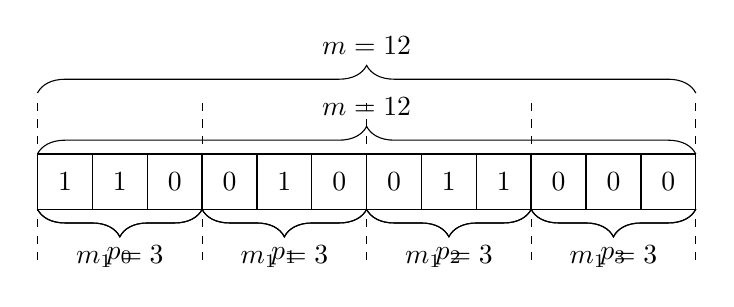
\begin{tikzpicture}
  \matrix (tape) [table, text width=7mm, name=tape]
    { 1 & 1 & 0 & 0 & 1 & 0 & 0 & 1 & 1 & 0 & 0 & 0 \\};

  \node[above=of tape-1-1.west] (s1) {};
  \node[below=of tape-1-1.west] (s2) {};

  \node[above=of tape-1-3.east] (s3) {};
  \node[below=of tape-1-3.east] (s4) {};

  \node[above=of tape-1-6.east] (s5) {};
  \node[below=of tape-1-6.east] (s6) {};

  \node[above=of tape-1-9.east] (s7) {};
  \node[below=of tape-1-9.east] (s8) {};

  \node[above=of tape-1-12.east] (s9) {};
  \node[below=of tape-1-12.east] (s10) {};

  \uncover<2-2>{\draw[brace] (tape-1-12.north east) -- node[yshift=6mm] {$m = 12$} (tape-1-1.north west);}
  \uncover<3->{\draw[brace] (s9.center) -- node[yshift=6mm] {$m = 12$} (s1.center);}

  \uncover<3->{
    \draw[dashed] (s1) to (s2);
    \draw[dashed] (s3) to (s4);
    \draw[dashed] (s5) to (s6);
    \draw[dashed] (s7) to (s8);
    \draw[dashed] (s9) to (s10);
  }

  \uncover<3-3>{
    \draw[brace] (tape-1-1.south west) -- node[yshift=-6mm] {$m_{1} = 3$} (tape-1-3.south east);

    \draw[brace] (tape-1-4.south west) -- node[yshift=-6mm] {$m_{1} = 3$} (tape-1-6.south east);

    \draw[brace] (tape-1-7.south west) -- node[yshift=-6mm] {$m_{1} = 3$} (tape-1-9.south east);

    \draw[brace] (tape-1-10.south west) -- node[yshift=-6mm] {$m_{1} = 3$} (tape-1-12.south east);
  }
  \uncover<4-4>{
    \draw[brace] (tape-1-1.south west) -- node[yshift=-6mm]  {$p_{0}$} (tape-1-3.south east);

    \draw[brace] (tape-1-4.south west) -- node[yshift=-6mm]  {$p_{1}$} (tape-1-6.south east);

    \draw[brace] (tape-1-7.south west) -- node[yshift=-6mm]  {$p_{2}$} (tape-1-9.south east);

    \draw[brace] (tape-1-10.south west) -- node[yshift=-6mm] {$p_{3}$} (tape-1-12.south east);
  }
\end{tikzpicture}
}
\end{frame}

\begin{frame}
  \frametitle{Tape simulation via pebbles}
  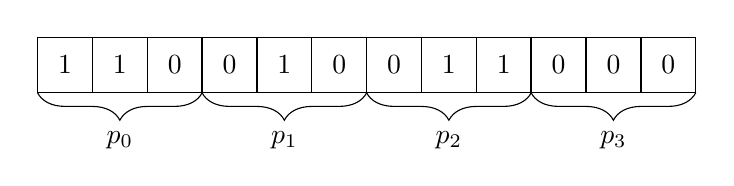
\begin{tikzpicture}
  \matrix (tape) [table, text width=7mm, name=tape]
    { 1 & 1 & 0 & 0 & 1 & 0 & 0 & 1 & 1 & 0 & 0 & 0 \\};
  \draw[brace] (tape-1-1.south west) -- node[yshift=-6mm] {$p_{0}$} (tape-1-3.south east); 
  \draw[brace] (tape-1-4.south west) -- node[yshift=-6mm] {$p_{1}$} (tape-1-6.south east); 
  \draw[brace] (tape-1-7.south west) -- node[yshift=-6mm] {$p_{2}$} (tape-1-9.south east); 
  \draw[brace] (tape-1-10.south west) -- node[yshift=-6mm] {$p_{3}$} (tape-1-12.south east); 
\end{tikzpicture}

  \begin{columns}
    \column{0.5\textwidth}
    \begin{itemize}
      \item Every pebbles needs $2^{m_{1}}$ distinct \enquote{states}
        \begin{itemize}
          \item Use placement on a walk with at least $2^{m_{1}}$ distinct vertices
        \end{itemize}
    \end{itemize}
    \column{0.5\textwidth}
    \resizebox{\textwidth}{!}{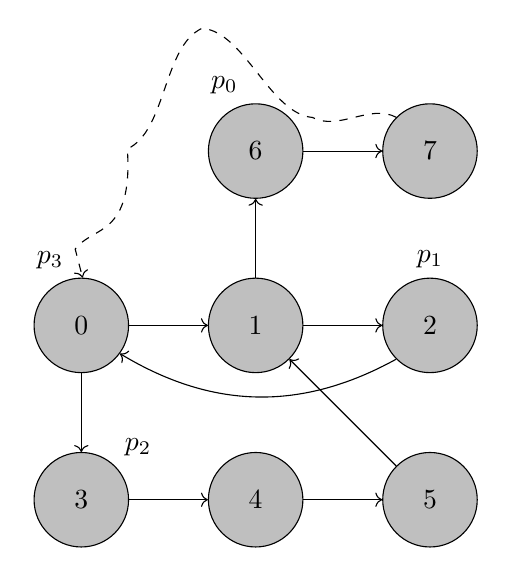
\begin{tikzpicture}
  \node[minimum size=12mm,inner sep=0mm, circle] (8) {};
  \node[node,right=of 8,label={100:$p_{0}$}] (6) {$6$};
  \node[node,right=of 6] (7) {$7$};
  \node[node,below=of 8,label={100:$p_{3}$}] (0) {$0$};
  \node[node,below=of 6] (1) {$1$};
  \node[node,below=of 7,label={$p_{1}$}] (2) {$2$};
  \node[node,below=of 0,label={45:$p_{2}$}] (3) {$3$};
  \node[node,below=of 1] (4) {$4$};
  \node[node,below=of 2] (5) {$5$};

  \draw[move] (0) to (1);
  \draw[move] (1) to (2);
  \draw[move,bend left] (2.south west) to (0);
  \draw[move] (0) to (3);
  \draw[move] (3) to (4);
  \draw[move] (4) to (5);
  \draw[move] (5) to (1);
  \draw[move] (1) to (6);
  \draw[move] (6) to (7);
  \draw[dashed, move, decorate,
  decoration={snake,amplitude=0.5cm, segment length=3cm}, bend right=55]
  (7.north west) to (0);
\end{tikzpicture}
}
  \end{columns}
\end{frame}

\end{document}
